\chapter[SCP-123 微型黑洞]{
    SCP-123 Contained Miniature Black Hole\\
    SCP-123 微型黑洞
}

\label{chap:SCP-123}

\begin{figure}[H]
    \centering
    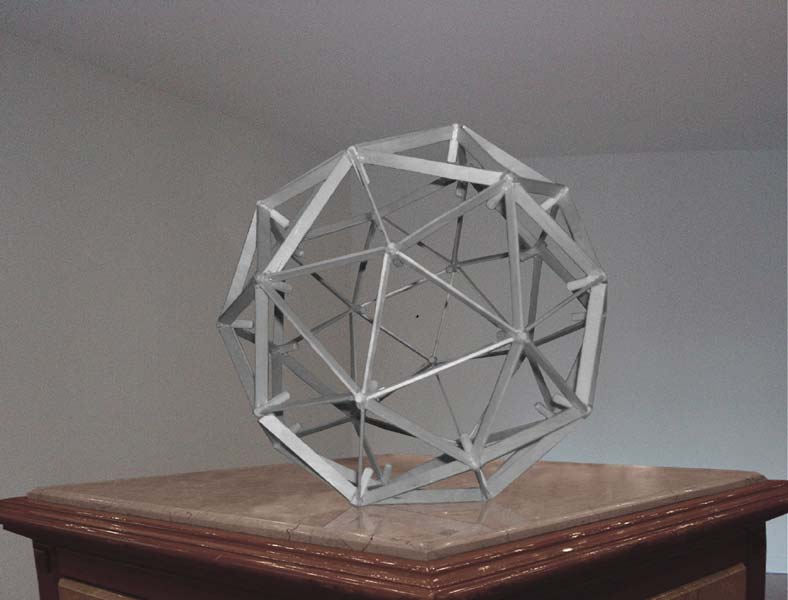
\includegraphics[width=0.5\linewidth]{images/SCP-123.jpg}
    \caption*{被合适地安置在桌上后很短时间内拍摄的SCP-123}
\end{figure}

\bb{项目编号:}SCP-123

\bb{项目等级:}Euclid

\bb{特殊收容措施:}SCP-123应被置于一个安全的设施内,用皮带、铁链、网或类似装置紧缚在一张紧固结实的桌子顶部。绝对不应用钩子固定装置。对象和桌子应置于一个不小于5mX5mX5m的房间中央。不应在SCP-123周围100米使用敏感测量设备,因为它们的测数会被明显影响。更重要的一点是除非进行试验,绝对禁止将任何物体放入SCP-123内。

SCP-123的转移应及其谨慎地进行,并且努力防止对象被摇晃或被大力击打。SCP-123在任何情况下都不得以任何手段运送至大型水体中。

2级以下人员禁止进入SCP-123的收容室。任何与对象进行接触的人员都应穿着紧身衣,完全没有肩带,鞋带或其他悬挂部分。长发人员应被要求向后束起头发或带发网。

\bb{描述:}对象是一个灰色测地线球体,直径65厘米,包括60个三角形。这些三角形之间的区域是空的,使得球心可见。球体材料未知,并且在█████博士建议下对于材料成分的研究应仅限于视觉观察,直到进一步通知。SCP-123似乎重约3.62公斤,尽管认为其实际质量要高得多。

测地线球体是中空的,除了正中心。在SCP-123的中心似乎是一个黑色球体,直径约1毫米。没有观察到从球体中反射出或发出任何光线。核心也表现出强大的引力,并且大幅增强了外部测地线球体的范围内的重力。这种引力可以被敏感仪器在几十米远外测量到。在大约三米内,对任何观察者引力的牵引都很明显,悬挂的物件开始被拉向球体。在外部球体的表面上,对于放置在球体上的物体引力达到其重量的两倍。

小物体被送入外部球体时内部球体的特性将会显现。任何此类物体都会迅速加速进入对象并且消失。任何注入的对象的液体也被吸进中央球体。分析显示黑色球体附近的光被弯曲转向中心。内部球体在其表面展现出的重力表明它的重量大约1029公斤,不过在外部球体内明显的重力削减效应意味着其真正质量或许远远超过。注意这样的质量通常意味着200米的史瓦西半径,超过实际观察到的约0.5毫米,可以认为是进一步证明了外部球体的重力抑制特性。

气体也受到SCP-123的重力影响,并且经测量其表面的大气压力为205千帕。然而气体无法穿越外部球体三角形之间的区域。原因目前未知,正在研究。

应该指出的是外部球体和内部球体似乎是共同体——每当外部球体移动时,内部球体亦然。建议进一步研究这种联系的特性。

\bb{附录{[}SCP-123a]:}SCP-123已经被视为一个废物处理器。目前负责SCP-123的研究员,█████博士,表示了对测地线球体结构完整性的担忧。所有废物处理请求必须经过█████博士或申请一个4级人员听证会。直到进一步通知前,所有与SCP-123的交互都应仅限于实验。指挥人员同意关于外部球体的耐久性还须进一步研究。
